
\chapter{Acceptance test}\label{ch:Test}

In this phase of the project, a series of tests will be performed, in order to find out if the solution can fulfill the set requirements.\\ 
All the videos and photos of the test's can be found in \ref{Ch:AppendixA}, and in the attached zip-files.

\section{Test 1 - Cycle time}

\paragraph{Testing Requirement 1:} The cycle time of the rotor must not exceed 26 seconds.\\
In order to test this requirement, the cycle time of the first half of the entire process is tested with the UR5. The cycle in this test therefore consists of moving the rotor from the conveyor belt to the balancing machine, then on to the visual inspection, and at last place it on the queue table. Since this is only half the steps of the entire process see \ref{fig:first-part}, this cycle is expected to be performed in 13 seconds or less. 

\subsubsection{Setup of the test}

\begin{itemize}
   \item A test rotor.
   \item A wooden frame simulating the drawer in the balancing machine.
   \item A fixture to simulate a hole in the queue table for the rotor to be placed in.
   
\end{itemize}

\paragraph{Expected outcome:}
The UR5 moves the rotor to each required point in 13 seconds or less. 

\paragraph{Results:}
The UR5 moved the rotor from the conveyor belt to each required position in approximately 13 seconds. 

\paragraph{Video link: }
See appendix \cite{testfilm}


\section{Test 2 - Ergonomics and signals.}

In this test the group will test the UR5 ability to react upon signals from the visual inspection, while keeping the work-flow intact.\\
Testing Requirements, see \ref{ch:Delimitations}:

\paragraph{Requirement 2:} It is required that the cobot differentiates the height of the rotor for visual inspection every hour. so the visual inspector is guided up from the static position throughout the entire workday.
\paragraph{Requirement 6:} The UR5 has to perform different task depending on signals it is receiving.
\subsubsection{Setup of the test}

The group made the UR5 move by coding an if-else loop. The main loop consisted of differentiating places of the rotor to be inspected, respectively 12 and 42 cm's above the table, so that the worker would switch between sitting and standing up depending on the height the rotor is being held.\\
When the button was pressed, this would take the UR5 into a different trajectory, which would mimic when a rotor failed the inspection.

\begin{itemize}
    \item 1  rotor.
    \item A button to emulate a signal from a machine.
    \item 2 objects at different heights. 
\end{itemize}

\paragraph{Expected outcome:} 
The UR5 is expected to lift the rotor from a height of 12 to 42 cm over the visual inspection table every 10. time, while a inspector will press a signal to move the rotor to the trash pile. 

\paragraph{Results: }

The worker was guided up in a position where he couldn't sit down, and then to a position where he could rest.\\
When the rotor failed, a new trajectory was taken by the UR5, and the rotor was then "failed". The UR5 would quickly find its starting point again and begin the sequence all over.\\

\paragraph{Video link: }
See appendix \cite{testfilm}

\section{Test 3 - Emergency stop}

When an emergency stop is pressed the UR5 should stop entirely.\\
Testing Requirements, see  \ref{ch:Delimitations}:\\

\paragraph{Requirement 3:} The emergency stops has to stop the entire work-cell.\\

\subsubsection{Setup of the test}

\begin{itemize}
    \item UR 5.
    \item The UR 5 teach pendant.
    \item 1 emergency stop.
\end{itemize}

\paragraph{Expected outcome:}
The manipulator will stop completely when pressing the emergency-stop.

\paragraph{Results: }
When the emergency stop on the teach pendant was activated, the manipulator stopped its trajectory. Before the manipulator could move again it was required to reset the emergency stop and teach pendant needed to be pushed.\\

\paragraph{Video link: }
See appendix \cite{testfilm}

\section{Test 4 - Multiple emergency stops}
The work-cell is a potentially dangerous environment to anyone entering it. The robots move around sharp rotors that could potentially cause injuries, despite the earlier mentioned safety measures. For this reason, it has been decided that an emergency stop button will be placed within reach of the employee performing the visual inspection.
\begin{figure}[H]
    \centering
    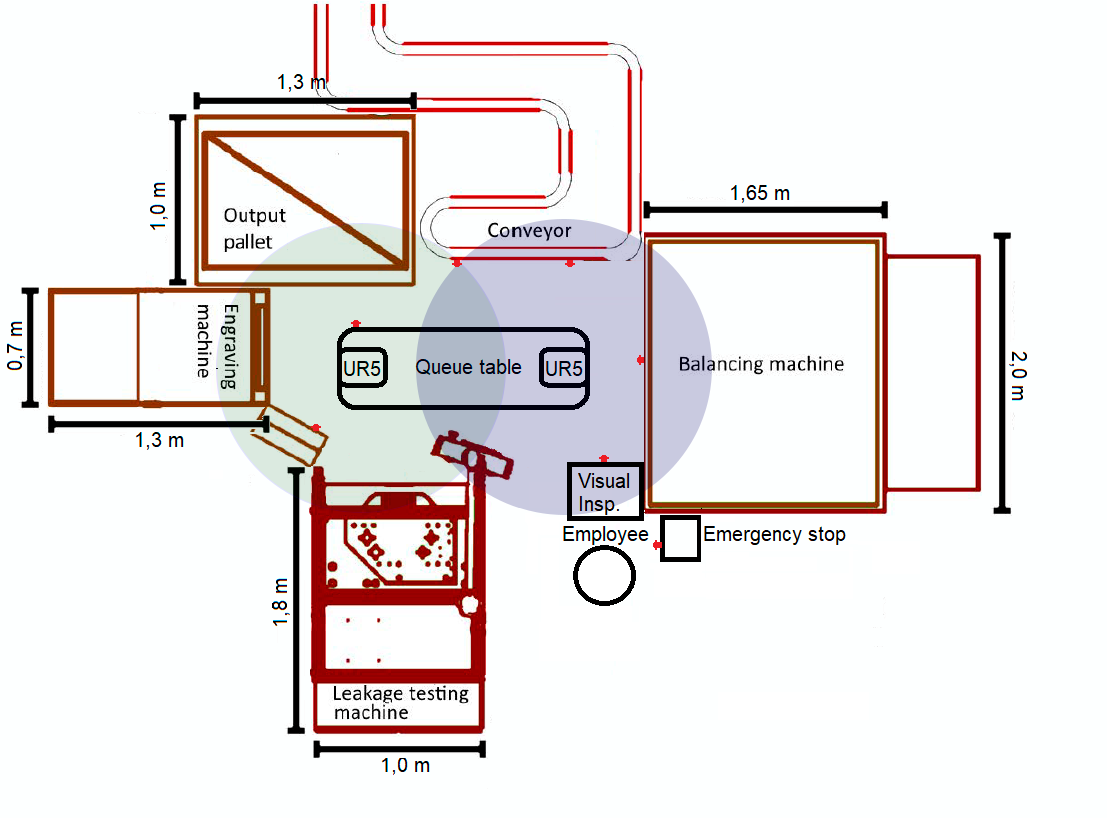
\includegraphics[width=0.7\textwidth]{Design/Work_cell_10.png}
    \caption{Illustration for the fourth test.}
    \label{fig:fourthtest}
\end{figure}
Additionally, 7 emergency stop buttons are strategically placed inside the work-cell see \ref{fig:fourthtest}, so that the distance from the nearest emergency stop button is maximum 55 cm from anywhere inside the work-cell. When an emergency stop is pressed, the UR5 will stop entirely. With this setup, anyone inside the work-cell would be able to immediately stop the production, if any emergency situation should occur. \\
\subsection{Setup of the test}
The test will be performed by making a button emulate an external emergency stop, this will connected to the safety input on the UR5 which are mark in yellow.

 \begin{itemize}
     \item UR5
     \item button
 \end{itemize}
 
 \paragraph{Expected outcome:}
The UR5 will stop completely when the emulated emergency stop is pushed

 
\paragraph{Results: }

The external emergency stop worked as expected, it stop the UR 5's process.

\paragraph{Video link: }
See appendix \cite{testfilm}


\section{Test 5 - Payload}
The purpose of this test is to verify that the UR5 is able to carry the required payload of 1145 grams. In order to test this, the UR5 must pick up and hold an object of the required weight in its most stretched out position.

\paragraph{Testing requirement 5:} The UR5 must be able to have a lifting capacity more than the total combined payload of the rotor(645g) and the end-effector(500g) at maximum reach.\\

\subsection{Setup of the test}
The test will be performed by making the UR5 pick up a block of iron(1530.9g) with the end-effector(500g). This will give a combined payload of 2030,9g. The UR5 will then move outward until it is holding the block at its maximum reach. 

 \begin{itemize}
     \item UR5
     \item Object weighing at least 1530.9g.
     \item End-effector 500g.
 \end{itemize}
 
 \paragraph{Expected outcome:}
The UR5 will pick up the block of iron and move it outward until it is at its maximum reach. 

 
\paragraph{Results: }
The UR5 was successful in performing the test. It is therefore concluded that the UR5 can handle the required payload.\\ 

\paragraph{Video link: }
See appendix \cite{testfilm}

\section{Test 6 - End-effector velocity}
When a worker enters the work-cell, the UR5's End-effector must not exceed 100mm/sec.

Testing Requirements, see  \ref{ch:Delimitations}:

\paragraph{Requirement 7:} When a worker enters the work-cell, the velocity of the end-effector on the UR5 has to slow down to 0,1 m/s, to reduce the risk of harmful behaviour.\\

\subsubsection{Setup of the test}
The velocity of the end-effector at the  300mm/s setting and 100 mm/s setting will be measured by tracking the motion off the end-effector, by recording the motion, with the use of a tracking software.
\begin{itemize}
    \item Measurement paper.
    \item 1 button.
    \item 1 camera
    \item Tracker software.
\end{itemize}

\paragraph{Expected outcome:}
The manipulator will slow down from 300 mm/s to 100 mm/s when the button is pressed.

\paragraph{Results: }
shows that the velocity at 300 mm/s had a maximum velocity at 350mm/s. The 100m/s had a maximum velocity of 130mm/s, see figure \ref{fig:velocitytest}.\\
This did not meet the expectations of the group, however the noise graph comes to the lack of having a good enough camera to produce a clear picture of the motion and may have yielded a better result. To meet the requirement of a maximum velocity of 100 mm/s, a lower velocity than 100mm/s will be used to make sure that the end-effector do not surpass the requirement.\\ 

\begin{figure}[H]
  \centering
    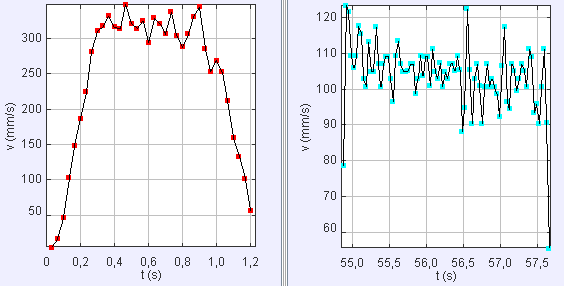
\includegraphics[width=\textwidth]{Design/velcit.PNG}
    \caption{The velocity of the end-effector at 300mm/s setting on the left and on the right 100mm/s setting}  \label{fig:velocitytest}
\end{figure}

\paragraph{Video link: }
See appendix \cite{testfilm}

\section{Test 7 -Accuracy and repeatability}
In this test, item number 8 from the delimitation will be tested. It is important in this pick and place scenario to place the rotor in the correct place every time. 

\subsubsection{Setup of the test}

\begin{itemize}
 \item 2 pieces of paper with circles 
 \item A pen 
\end{itemize}

The UR 5 will be programmed in a loop to make a dot ten times within the circles on each paper. After that it will be measured to make sure that it is within the requirements.

\paragraph{Expected outcome:}
Due to the specifications on the UR5, which has a repeatable accuracy of 0.1mm. The exceptions for the this test is that any of the dots is inside a radius of 0.1mm.

\paragraph{Results: }
Shows that the UR5 could perform the task of being accurate within 0.1mm and upheld the requirements of being within the radius of 1mm. 

\paragraph{Video link: }
See appendix \cite{testfilm}



%\section{Test 5: }
\section{Test discussions}
In this section, each of the requirements will be discussed. 

\paragraph{Requirement 1:}
The test was successfully completed in 13 seconds. This might indicate that the total cycle time is plausible to complete in 26 seconds or less. However, the test did not include the processing time in the balancing machine and visual inspection. 

\paragraph{Requirement 2+6:}
Taken in to consideration, that worker who operates the work-cell, is of different heights, a variable setup of the visual station might be needed. So that the ergonomics will apply to all the workers.\\
The signal needs to be implemented in the program, so whenever the signal is pressed the rotor will be moved in to a different trajectory.\\
It is assumed that this test is enough for testing the signals, since it is the same concept.

\paragraph{Requirement 3:}
It was expected that the UR5's emergency stop would work, since it is an integrated part of the system from Universal Robots. 

\paragraph{Requirement 4:}

The test of requirement of having more the just one emergency stop within the work-cell was test with only one external emergency stop. The fact that emergency stop by having a NC(normally closed) switch, that when the switch is activated it is open so that there is no continuity, the team expects that if all the emergency stops is connected in series, so if one is activated it effects the entire work-cell.  

\paragraph{Requirement 5:}
The UR5 was able to lift more than the required payload out to its maximum reach. This indicates that it will be able to lift the lighter rotor around into every required position at high speeds without breaking. This was expected since the stated payload of the UR5 is 5 kg. 


\paragraph{Requirement 6:}
The graph of the end-effectors velocity did show 30mm/s too fast, which can be for  two reasons. The first is that it could be due to the lack of a professional camera, that had higher resolution than an IPhone. The group only processed mobile-phones and a mobile phone is not a professional choice.\\
The other reason could be that the different velocities of the different joints would accelerate the end-effector, when starting and stopping. 


\paragraph{Requirement 7:}
In the test, it was possible to reduce the speed of the robot by simulating the light curtain sensor with a button. This indicates that it would be possible to implement a light curtain sensor, which could slow down the UR5 to the required speed. 


\paragraph{Requirement 8:}
The UR5 was able to hit the center of the circle 10 times with a deviation of less than 0,1 mm. This reinforces the stated maximum deviation on the UR5 of 0,1 mm. 
 

 